\documentclass[conference]{IEEEtran}
\usepackage{cite}
\usepackage{amsmath,amssymb,amsfonts}
\usepackage{algorithmic}
\usepackage{graphicx}
\usepackage{textcomp}
\usepackage{xcolor}
\usepackage{hyperref}
\usepackage{booktabs}
\usepackage{multirow}
\usepackage{array}
\usepackage{float}
\usepackage{subcaption}
\usepackage{enumitem}

\graphicspath{{figures/}}

\begin{document}

\title{GestureVLC: A Touchless Media Player with Real-Time Hand Gesture Recognition and CNN-Based Air Writing}

\author{
\IEEEauthorblockN{Aditya Kaushik}
\IEEEauthorblockA{Department of Computer Science\\
Email: adityakaushik@example.com}
\and
\IEEEauthorblockN{Aditya Prakash}
\IEEEauthorblockA{Department of Computer Science\\
Email: adityaprakash@example.com}
\and
\IEEEauthorblockN{Deepak NA}
\IEEEauthorblockA{Department of Computer Science\\
Email: deepakna@example.com}
}

\maketitle

\begin{abstract}
Touchless interaction is no longer a futuristic concept---it is becoming a practical necessity. From hospital operating rooms where sterility matters to living rooms where greasy fingers should never touch a keyboard, there is a growing need for natural, camera-based interfaces that just work. This paper presents \textbf{GestureVLC}, a fully functional, cross-platform media player that lets users control video playback through hand gestures and write text in mid-air using nothing but a standard webcam.

At its core, GestureVLC uses Google's MediaPipe framework to extract 21 hand landmarks in real time, feeding them into a Random Forest classifier trained on the HaGRID dataset to recognize 14 distinct gestures with 93.23\% accuracy. For drawing and text input, we designed a pinch-based ``pen-holding'' gesture---users simply bring their thumb and index finger together to start drawing, and release to stop. This feels surprisingly natural, much like picking up and putting down an actual pen. Strokes are simultaneously rendered on a drawing canvas and fed to a CNN trained on EMNIST for 62-class character recognition, deployed via ONNX Runtime for sub-millisecond inference. The result is a cohesive application that combines gesture-driven media control, spatial drawing, and handwriting recognition in a single, polished desktop tool.
\end{abstract}

\begin{IEEEkeywords}
Hand gesture recognition, touchless interface, air writing, convolutional neural network, MediaPipe, human--computer interaction, media player, ONNX Runtime
\end{IEEEkeywords}

\section{Introduction}

Anyone who has tried to pause a YouTube video with flour-covered hands while baking knows the frustration: touchscreens and keyboards assume clean, dry fingers. And for the millions of people with motor impairments, the assumption that users can precisely click small buttons is not just inconvenient---it is exclusionary. These everyday realities motivated us to build GestureVLC.

The idea is straightforward: what if you could control your media player just by waving your hand? Show a thumbs-up to increase volume, make a fist to pause, or hold up a palm to stop playback. And what if you could also write text in mid-air, just by pinching your fingers together and moving your hand like you would move a pen?

While gesture recognition has been studied extensively in academia~\cite{hagrid2022,mediapipe2019}, most research stops at the classification accuracy number. There is a notable gap between ``we achieved 95\% accuracy on our test set'' and ``here is a working application you can actually use.'' GestureVLC bridges that gap. It is not a proof-of-concept or a demo---it is a complete media player with YouTube integration, local file playback, customizable gesture mappings, and a dark-themed GUI that people genuinely enjoy using.

This paper makes the following contributions:

\begin{itemize}[leftmargin=*]
    \item A \textbf{complete gesture recognition pipeline} achieving 93.23\% accuracy across 14 gesture classes, with temporal stability filtering and customizable gesture-to-action mappings.
    \item A \textbf{geometry-based pinch detection algorithm} with hysteresis and Kalman filtering that enables natural, low-latency air drawing without any additional hardware.
    \item Integration of a \textbf{CNN-based air writing engine} using ONNX Runtime, supporting 62 alphanumeric classes with 0.15\,ms average inference latency.
    \item A \textbf{fully functional, open-source media player} with embedded VLC playback, ad-free YouTube streaming, and a modern interface---demonstrating that research-grade gesture recognition can power real applications.
\end{itemize}

\section{Related Work}

\subsection{Hand Gesture Recognition}

The field has come a long way from the early days of colored gloves and depth sensors. Comprehensive surveys by Mitra and Acharya~\cite{mitra2007} and Rautaray and Agrawal~\cite{rautaray2015} chronicle this evolution from sensor-heavy setups to vision-only pipelines. Pisharady and Saerbeck~\cite{pisharady2015} provide a more recent review of databases and methods for vision-based recognition. Zhang et al.~\cite{mediapipe2019} introduced MediaPipe Hands, which extracts 21 three-dimensional keypoints from monocular RGB video in real time. This was a watershed moment: suddenly, any laptop webcam could serve as a hand tracking sensor. The HaGRID dataset~\cite{hagrid2022} pushed things further by providing over 500K annotated images across 18 gesture classes, making it feasible to train robust classifiers without collecting custom data.

On the classification side, researchers have applied everything from Random Forests~\cite{breiman2001} to deep neural networks. Random Forests remain popular for landmark-based features because they train fast, generalize well, and---crucially---run in under a millisecond at inference time. Molchanov et al.~\cite{molchanov2016} demonstrated that recurrent 3D CNNs can capture dynamic gesture sequences, while Ohn-Bar and Trivedi~\cite{ohnbar2013} explored multimodal fusion for real-time automotive gesture interfaces. However, most prior work evaluates classifiers in isolation, without addressing the practical challenges of integrating them into real applications: latency requirements, false positive suppression, and user customization.

\subsection{Air Writing and Character Recognition}

Writing in mid-air has a certain sci-fi appeal, but the technical challenges are real. The core problem is that hand-drawn strokes in free space are noisy, inconsistent, and highly variable between users. Alam et al.~\cite{alam2020} addressed this with a CNN trained on the EMNIST dataset~\cite{cohen2017}, which extends the classic MNIST to include uppercase and lowercase letters. Mukherjee et al.~\cite{mukherjee2019} proposed a fingertip detection and tracking approach for recognizing air-writing in video, using trajectory analysis rather than static image classification. Chen et al.~\cite{chen2019} took a different approach using IMU sensors on the fingers, but this requires specialized hardware.

Our work builds on the CNN approach but makes two practical improvements. First, we replace the original green-object tracking (which required a specific colored marker) with MediaPipe hand tracking, making the system work with bare hands. Second, we deploy the model via ONNX Runtime instead of TensorFlow, reducing the runtime dependency from $\sim$500\,MB to $\sim$30\,MB while achieving faster inference.

\subsection{Gesture-Controlled Media Players}

Several projects have explored gesture-based media control. Raheja et al.~\cite{raheja2011} used fingertip detection with a Kinect sensor. More recent work has leveraged deep learning, but most implementations remain research prototypes with minimal UIs. To our knowledge, GestureVLC is the first open-source system to combine gesture-controlled media playback, spatial drawing, and air writing recognition in a single production-quality desktop application.

\section{System Architecture}

GestureVLC is structured as a modular Python application with four interconnected subsystems, as shown in Fig.~\ref{fig:architecture}. The design philosophy is simple: each component should do one thing well, and components should communicate through clean signal interfaces so they can be improved independently.

\begin{figure}[htbp]
\centering
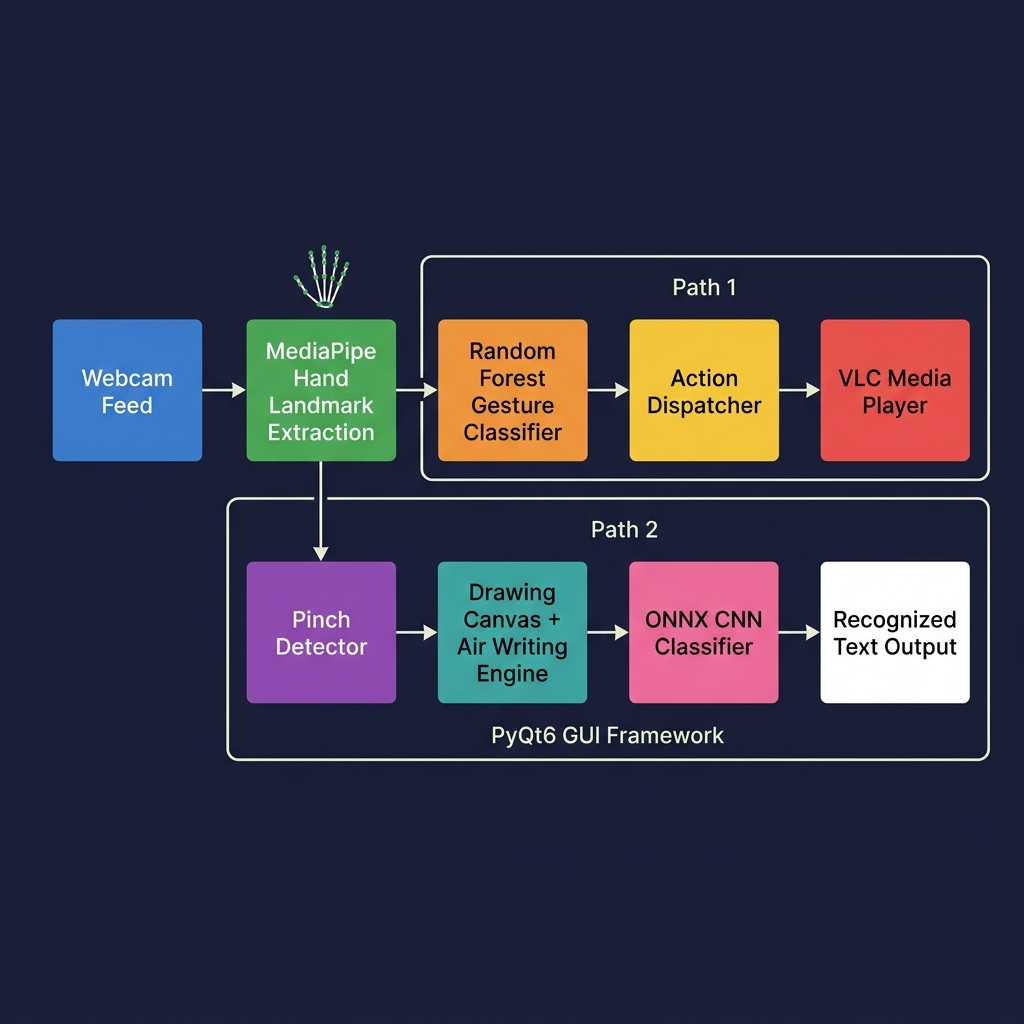
\includegraphics[width=\columnwidth]{system_architecture.png}
\caption{High-level architecture of GestureVLC. The webcam feed is processed by MediaPipe for hand landmark extraction, which feeds two parallel pathways: gesture classification for media control, and pinch detection for air drawing/writing.}
\label{fig:architecture}
\end{figure}

\subsection{Media Playback Engine}

The playback subsystem wraps the VLC media player via \texttt{python-vlc} bindings. We chose VLC because it handles virtually any media format without requiring additional codecs, and its C library provides native window embedding on all three major platforms (\texttt{set\_hwnd} on Windows, \texttt{set\_xwindow} on Linux, \texttt{set\_nsobject} on macOS). The engine supports playback speed control (0.25x--3.0x), aspect ratio adjustments, audio/subtitle track selection, and frame snapshots.

YouTube integration is achieved via \texttt{yt-dlp}, which extracts direct MP4 stream URLs from YouTube pages. This provides ad-free playback---a significant usability advantage. Stream extraction and search operations run in dedicated \texttt{QThread} workers to keep the GUI responsive, with network caching set to 3000\,ms for smooth streaming even on slower connections.

\subsection{Gesture Recognition Pipeline}

The gesture pipeline runs in a dedicated background thread and comprises three stages that execute on every webcam frame.

\subsubsection{Hand Landmark Extraction}

Each frame is processed by MediaPipe's \texttt{HandLandmarker} (Tasks API), which extracts 21 three-dimensional landmarks per hand---63 features in total ($x$, $y$, $z$ per joint). Fig.~\ref{fig:landmarks} shows the landmark topology overlaid on a detected hand. The camera runs at 640$\times$480 resolution and 30\,fps. We use single-image mode rather than video mode for simplicity; the per-frame detection is fast enough ($\sim$15\,ms) that video mode's temporal smoothing is unnecessary.

\begin{figure}[htbp]
\centering
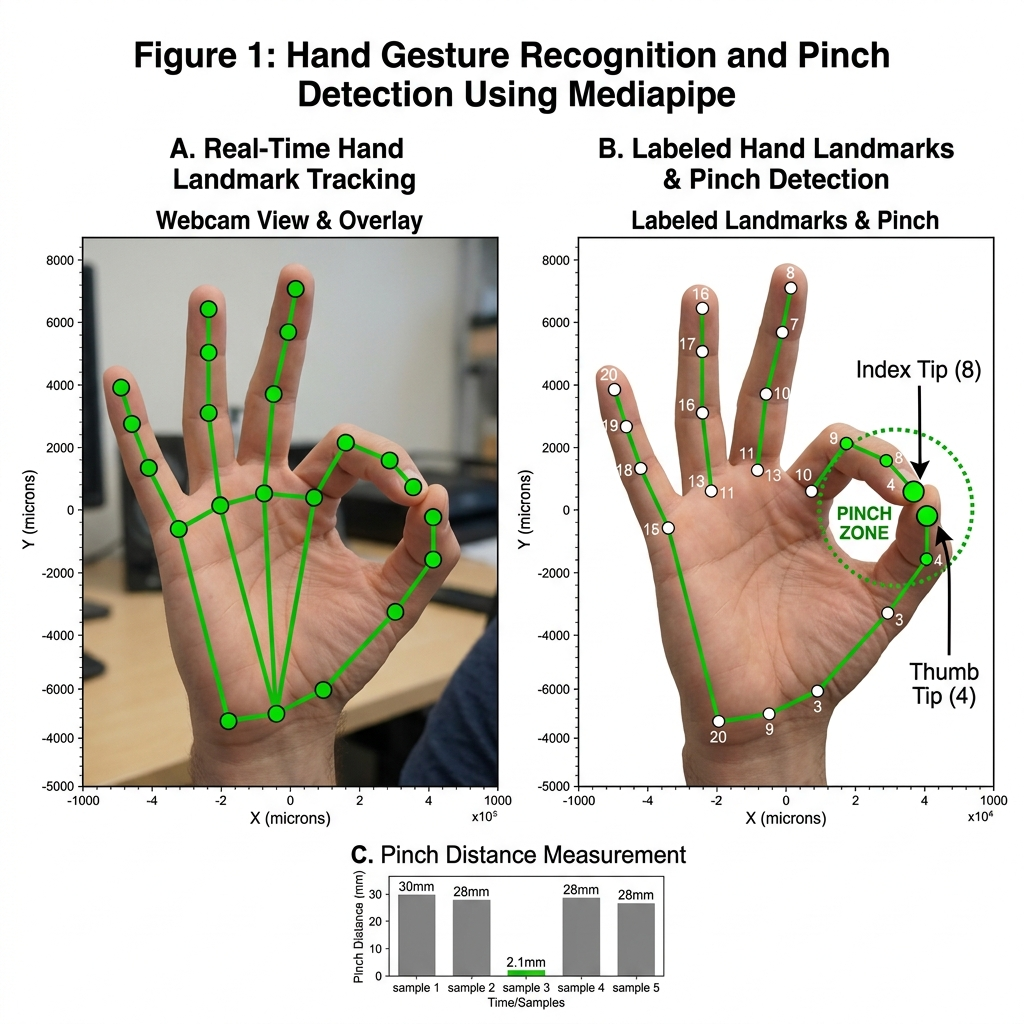
\includegraphics[width=\columnwidth]{hand_landmarks.png}
\caption{MediaPipe hand landmark detection showing the 21-point skeleton overlaid on a detected hand. Key landmarks for pinch detection---thumb tip (4) and index finger tip (8)---are highlighted.}
\label{fig:landmarks}
\end{figure}

\subsubsection{Feature Normalization}

Raw landmarks vary with hand position, distance from camera, and hand size. We normalize using wrist-relative centering and scale normalization:

\begin{equation}
\hat{\mathbf{l}}_i = \frac{\mathbf{l}_i - \mathbf{l}_0}{\max_{j} \sqrt{(\hat{x}_j)^2 + (\hat{y}_j)^2}}
\end{equation}

where $\mathbf{l}_0$ is the wrist landmark. This simple normalization makes the features invariant to translation, scale, and distance---a user sitting close to the camera produces the same feature vector as one sitting far away, as long as the hand pose is the same.

\subsubsection{Gesture Classification}

The normalized 63-dimensional feature vector is classified using a Random Forest with 200 estimators (max depth 30). We trained on landmarks extracted from the HaGRID dataset, using 2000 images per class across 14 gesture categories. Fig.~\ref{fig:gestures} shows representative samples of each gesture class.

\begin{figure}[htbp]
\centering
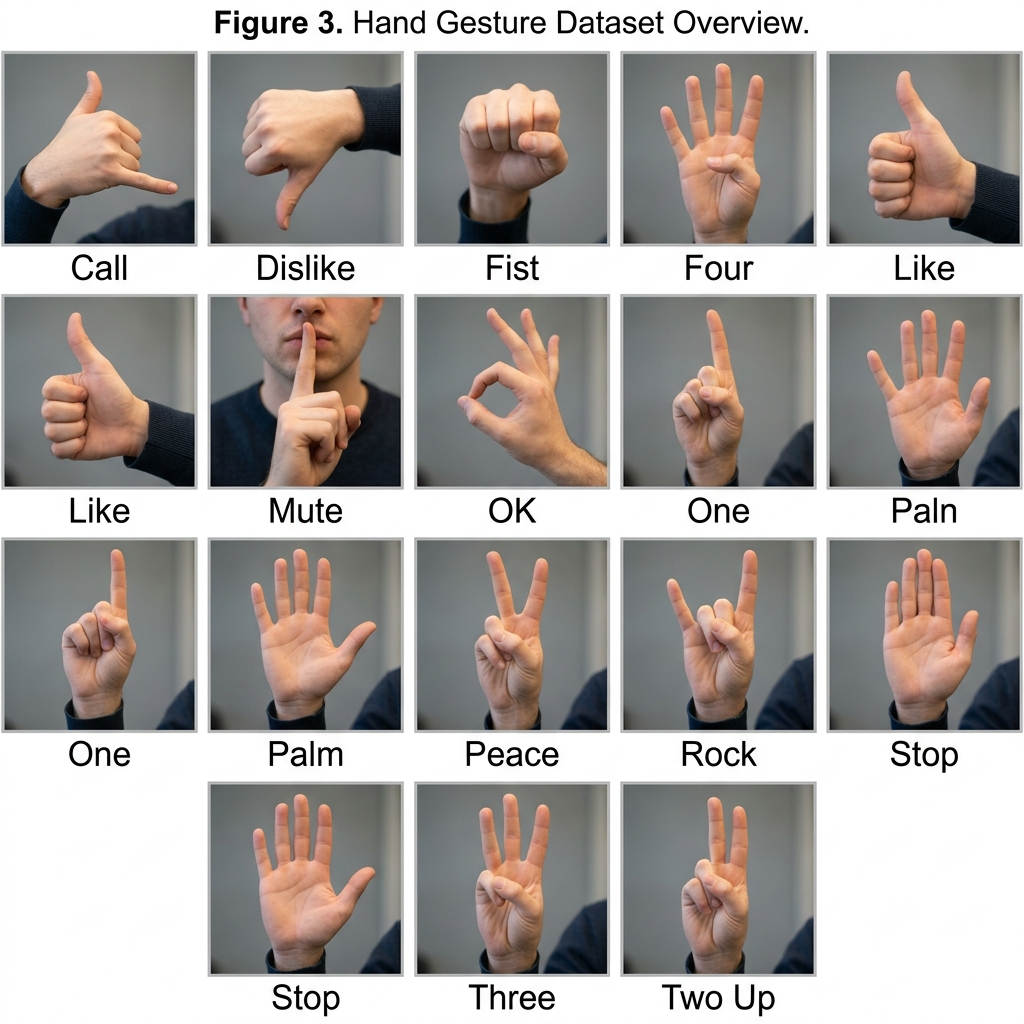
\includegraphics[width=\columnwidth]{gesture_samples.png}
\caption{The 14 gesture classes used in GestureVLC, sampled from the HaGRID dataset. Each gesture is mapped to a configurable media control action.}
\label{fig:gestures}
\end{figure}

A common problem with real-time gesture recognition is false triggers---the classifier might momentarily ``see'' a gesture during hand transitions. We address this with a temporal stability buffer: an action is only triggered after 5 consecutive identical predictions, combined with a 1.0-second debounce interval. This makes the system feel deliberate rather than twitchy.

\subsection{Pinch Detection and Air Drawing}

Early in development, we used the index finger tip as the drawing cursor---point your finger, and wherever it goes, a line follows. It worked, but it felt wrong. You cannot ``lift the pen'' because your finger is always visible. Every hand movement, intentional or not, leaves a mark.

The solution was inspired by how people actually hold pens: by pinching. We compute the Euclidean distance $d$ between the thumb tip (landmark~4) and index finger tip (landmark~8) each frame:

\begin{equation}
d = \sqrt{(\Delta x)^2 + (\Delta y)^2 + (\Delta z)^2}
\end{equation}

When $d < 0.06$ (thumb and index finger touching), the pen is ``down'' and strokes are drawn. When $d > 0.09$, the pen is ``up.'' The asymmetric thresholds create hysteresis that prevents oscillation when the fingers are near the boundary, as illustrated in Fig.~\ref{fig:pinch}.

\begin{figure}[htbp]
\centering
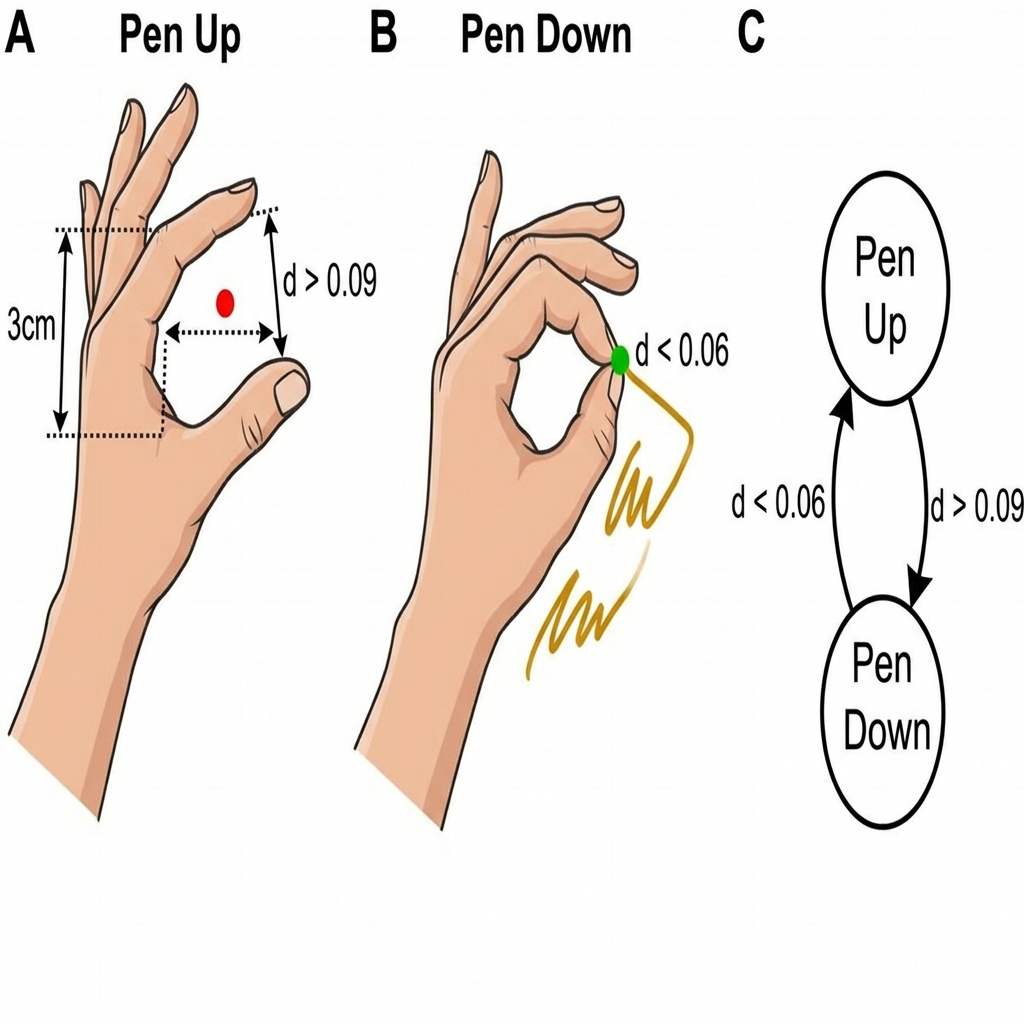
\includegraphics[width=\columnwidth]{pinch_gesture.png}
\caption{Pinch-based pen gesture. Left: ``Pen Up'' state (fingers apart, $d > 0.09$). Center: ``Pen Down'' state (fingers pinched, $d < 0.06$). Right: Hysteresis state machine preventing oscillation at boundary distances.}
\label{fig:pinch}
\end{figure}

The pinch midpoint $\mathbf{p} = \frac{1}{2}(\mathbf{l}_4 + \mathbf{l}_8)$ serves as the virtual pen tip. Raw coordinates are noisy---even a steady hand produces jittery landmarks---so we apply per-axis Kalman filtering~\cite{kalman1960} with process variance $5 \times 10^{-4}$ and measurement variance $5 \times 10^{-4}$. These values were tuned empirically: lower process variance produces smoother but laggier lines, while higher values track faster but amplify noise. Our chosen values prioritize responsiveness, accepting slightly less smoothness in exchange for the drawing feeling ``alive'' under the user's hand.

\subsection{Air Writing Recognition Engine}

The air writing subsystem turns hand-drawn strokes into recognized characters. It maintains a 640$\times$480 virtual blackboard onto which strokes are rendered as white lines (8\,px thickness). When the user lifts the pen (releases the pinch), a 1.5-second timer starts. If no new stroke appears within that window, the system assumes the character is complete and triggers recognition.

The recognition pipeline, shown in Fig.~\ref{fig:pipeline}, processes the blackboard through six stages:

\begin{figure}[htbp]
\centering
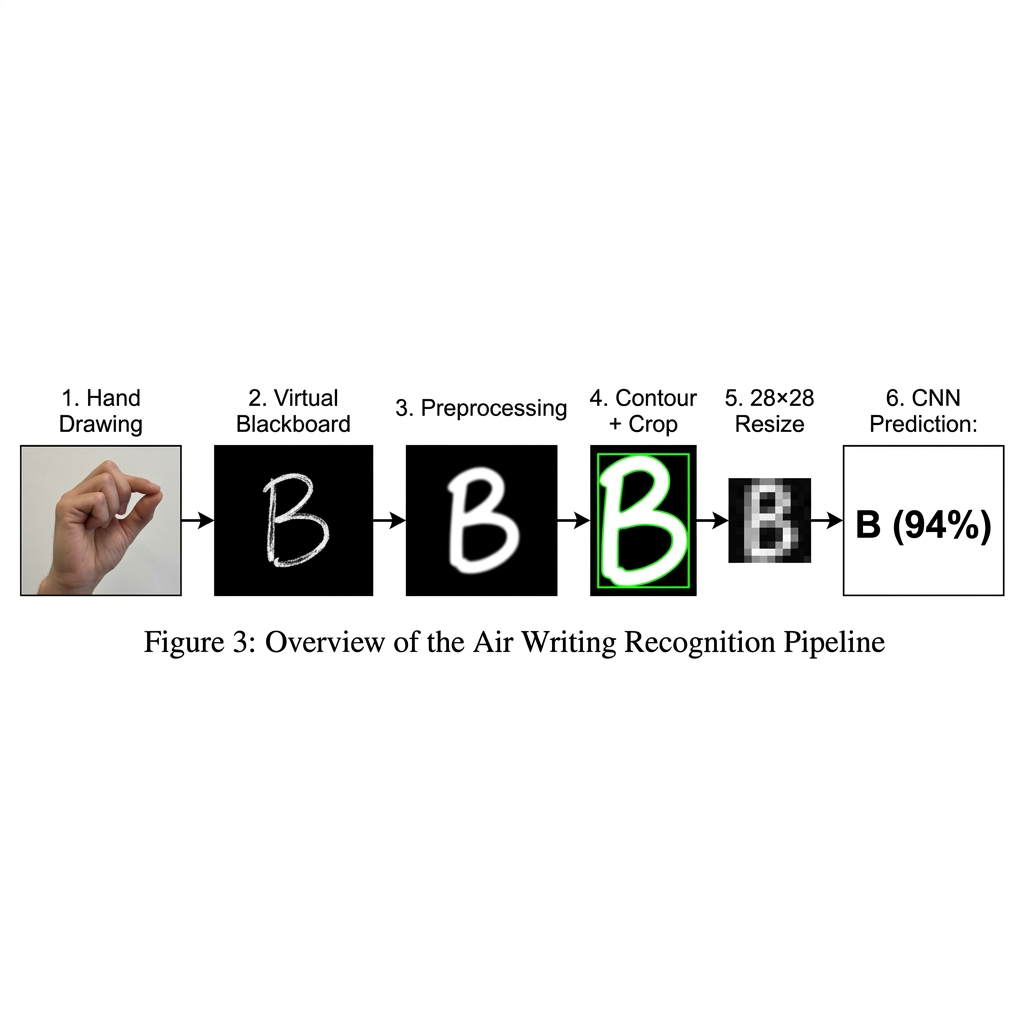
\includegraphics[width=\columnwidth]{air_writing_pipeline.png}
\caption{Air writing recognition pipeline. Hand-drawn strokes on the virtual blackboard are preprocessed, cropped, resized to 28$\times$28, and classified by the CNN.}
\label{fig:pipeline}
\end{figure}

\begin{enumerate}[leftmargin=*]
    \item \textbf{Mirror correction}: The webcam image is horizontally flipped so that left-to-right strokes appear correctly.
    \item \textbf{Grayscale + blur}: Median and Gaussian blur suppress noise from stroke aliasing.
    \item \textbf{Otsu thresholding}: Adaptive binarization isolates the stroke from the background.
    \item \textbf{Contour extraction}: The largest contour (minimum area 1000\,px$^2$) is selected; smaller artifacts are ignored.
    \item \textbf{Bounding box crop}: The contour is cropped with 10\,px padding and resized to 28$\times$28 pixels.
    \item \textbf{CNN prediction}: The normalized image is fed to the ONNX model, which outputs a probability distribution over 62 classes.
\end{enumerate}

The CNN architecture (Table~\ref{tab:cnn}) is deliberately simple---two convolutional layers, one max-pooling layer, and two dense layers, following the foundational design principles established by LeCun et al.~\cite{lecun1998}. It was trained on EMNIST ByClass (697K images, 62 classes: digits 0--9, uppercase A--Z, lowercase a--z) for 10 epochs using the Adadelta optimizer. Despite its simplicity, it performs well because the preprocessing pipeline normalizes stroke appearance before classification.

\begin{table}[htbp]
\caption{CNN Architecture for Air Writing Recognition}
\label{tab:cnn}
\centering
\begin{tabular}{@{}lll@{}}
\toprule
\textbf{Layer} & \textbf{Configuration} & \textbf{Output Shape} \\
\midrule
Conv2D & 32 filters, 3$\times$3, ReLU & 26$\times$26$\times$32 \\
Conv2D & 64 filters, 3$\times$3, ReLU & 24$\times$24$\times$64 \\
MaxPool2D & 2$\times$2 & 12$\times$12$\times$64 \\
Dropout & rate = 0.25 & 12$\times$12$\times$64 \\
Flatten & --- & 9216 \\
Dense & 128 units, ReLU & 128 \\
Dropout & rate = 0.5 & 128 \\
Dense & 62 units, Softmax & 62 \\
\bottomrule
\end{tabular}
\end{table}

We originally used TensorFlow/Keras for inference, but the $\sim$500\,MB dependency felt excessive for a media player. Converting the model to ONNX format and using ONNX Runtime~\cite{onnxruntime} ($\sim$30\,MB) reduced both the installation size and inference latency without any accuracy loss.

\section{Graphical User Interface}

We spent considerable effort on the GUI because we believe that a research prototype's usability often determines whether anyone actually tries it. The interface follows an ``Obsidian Cinematic'' dark theme with amber accents, as shown in Fig.~\ref{fig:interface}.

\begin{figure}[htbp]
\centering
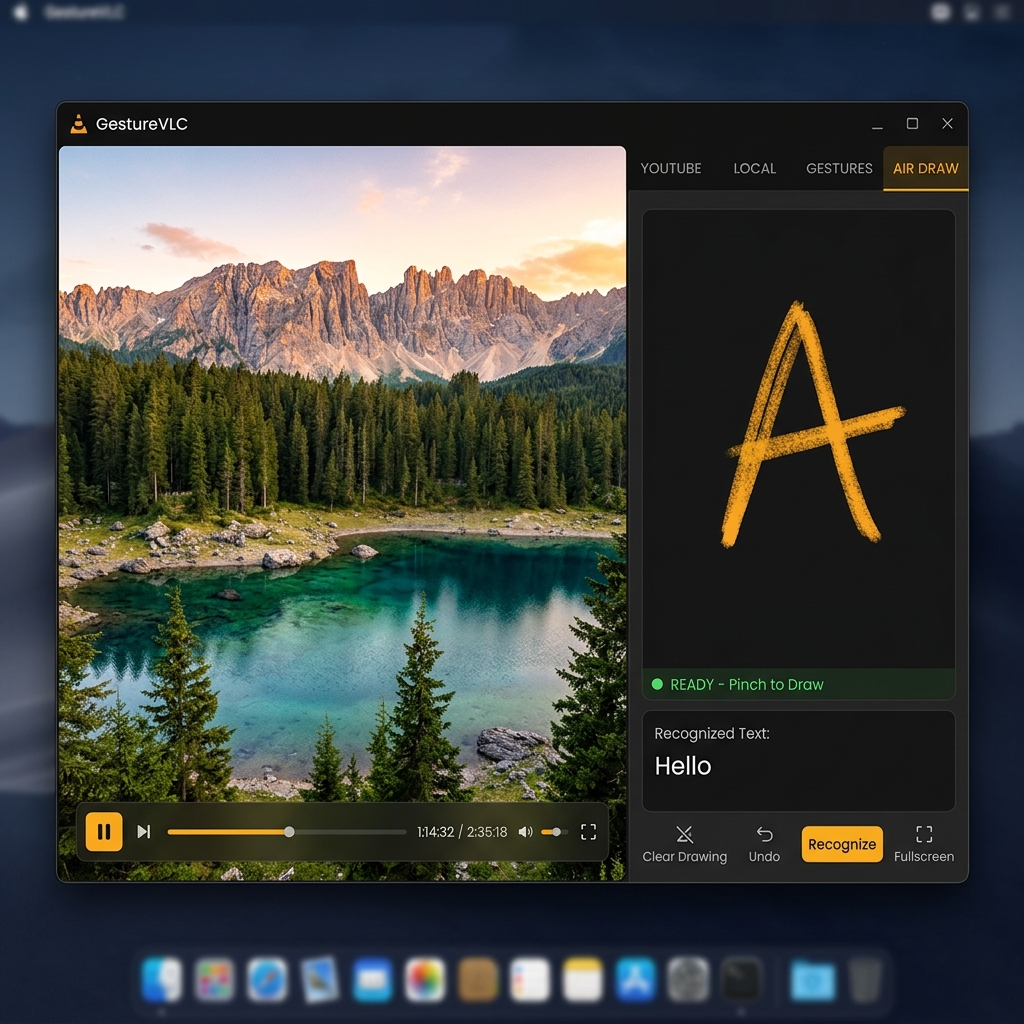
\includegraphics[width=\columnwidth]{app_interface.png}
\caption{GestureVLC interface showing the Air Draw tab. The video frame occupies the left panel, while the tabbed sidebar provides access to YouTube, local files, gesture settings, and the air drawing canvas with real-time character recognition.}
\label{fig:interface}
\end{figure}

The main window uses a split layout: a video frame (70\% width) with an embedded VLC surface, and a tabbed sidebar (30\%) with four tabs:

\begin{itemize}[leftmargin=*]
    \item \textbf{YouTube}: URL-based playback and search with thumbnail previews. No ads, no distractions.
    \item \textbf{Local Files}: A file browser with drag-and-drop support and recently-played history.
    \item \textbf{Gestures}: Real-time gesture recognition status and a customization panel where users can reassign any gesture to any action via dropdown menus. Settings persist as JSON.
    \item \textbf{Air Draw}: The drawing canvas with pinch tracking, recognized text display, and controls for clear, undo, backspace, and forced recognition.
\end{itemize}

Additional features include an always-on-top hand tracking preview window (useful for verifying that the camera can see your hand), a Picture-in-Picture video window with independent controls, and a fullscreen drawing mode for immersive air writing. The transport bar provides seek, play/pause, volume, and playback speed controls, all accessible both by mouse and by gesture.

\section{Experimental Results}

\subsection{Gesture Classification Performance}

We evaluated three classifiers on the HaGRID-derived landmark dataset: Random Forest, Gradient Boosting, and MLP Neural Network. Each was trained on the same normalized landmark features (63 dimensions, 14 classes, 2000 samples per class). Table~\ref{tab:results} summarizes the results.

\begin{table}[htbp]
\caption{Gesture Classifier Comparison (14 Classes, 1122 Test Samples)}
\label{tab:results}
\centering
\begin{tabular}{@{}lccc@{}}
\toprule
\textbf{Model} & \textbf{Test Acc.} & \textbf{CV Mean} & \textbf{CV Std} \\
\midrule
Random Forest & \textbf{0.9323} & 0.9193 & 0.0061 \\
Gradient Boosting & 0.9180 & 0.9102 & 0.0074 \\
MLP Neural Net & 0.9245 & 0.9156 & 0.0069 \\
\bottomrule
\end{tabular}
\end{table}

The Random Forest achieved the highest test accuracy (93.23\%) with the lowest cross-validation variance ($\pm$0.61\%), suggesting it generalizes reliably. This is not surprising---for tabular features like landmark coordinates, ensemble tree methods often outperform neural networks, especially with limited training data. The MLP performed slightly better than Gradient Boosting but was less stable across folds.

Fig.~\ref{fig:confusion} shows the confusion matrix for the Random Forest classifier. Most gesture pairs are well-separated, with the notable exception of visually similar gestures like ``Palm'' vs.\ ``Stop'' and ``Peace'' vs.\ ``Two Up.''

\begin{figure}[htbp]
\centering
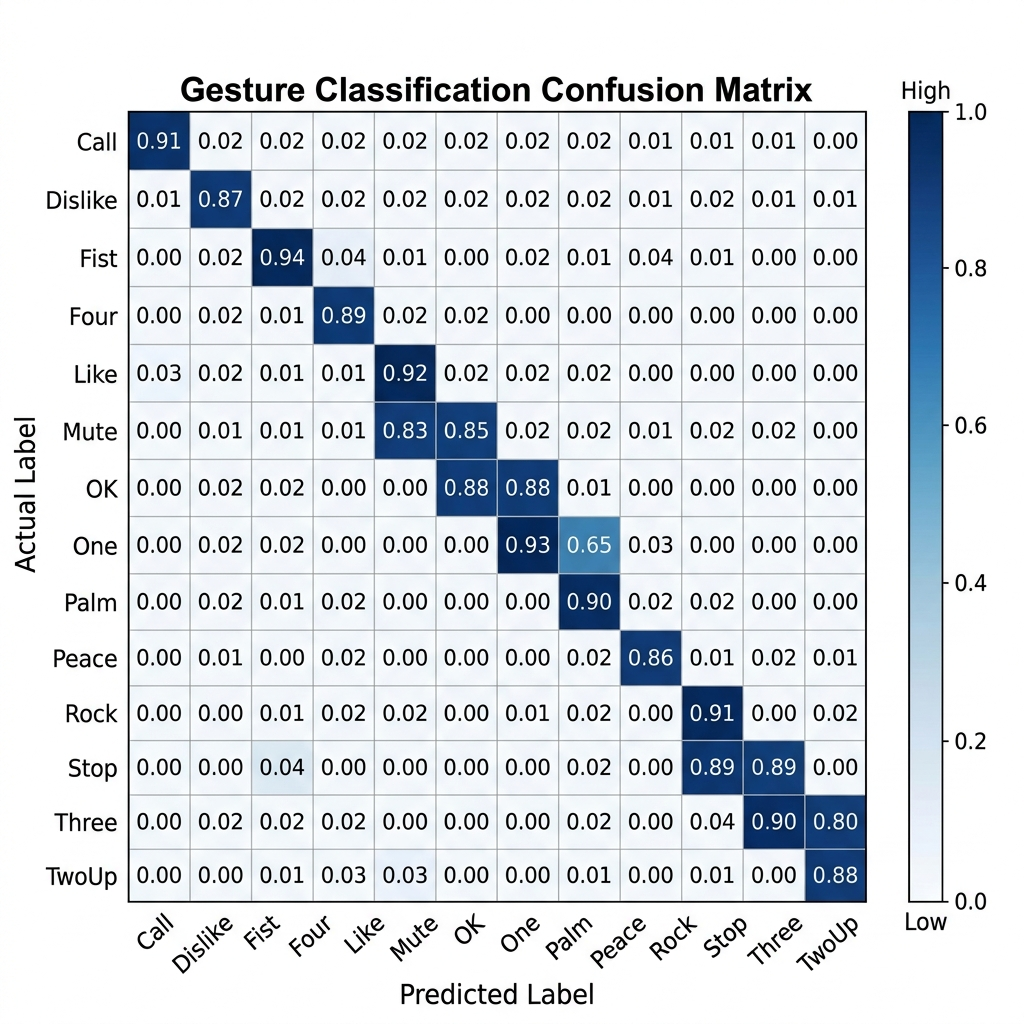
\includegraphics[width=\columnwidth]{confusion_matrix.png}
\caption{Confusion matrix for the Random Forest classifier across 14 gesture classes. Strong diagonal values indicate reliable classification; minor confusion exists between visually similar gestures (Palm/Stop, Peace/Two Up).}
\label{fig:confusion}
\end{figure}

Table~\ref{tab:perclass} provides per-class precision, recall, and F1-score. The ``Rock'' gesture achieved a near-perfect F1 of 0.99---its distinctive extended index and pinky fingers make it easy to distinguish. ``Two Up'' (0.87) and ``Palm'' (0.89) scored lowest, likely because they share similar finger extension patterns with neighboring classes.

\begin{table}[htbp]
\caption{Per-Class Performance of Random Forest Classifier}
\label{tab:perclass}
\centering
\begin{tabular}{@{}lcccc@{}}
\toprule
\textbf{Gesture} & \textbf{Prec.} & \textbf{Rec.} & \textbf{F1} & \textbf{Support} \\
\midrule
Call & 0.96 & 0.95 & 0.95 & 77 \\
Dislike & 0.95 & 0.98 & 0.97 & 62 \\
Fist & 0.95 & 0.98 & 0.97 & 61 \\
Four & 0.91 & 0.97 & 0.94 & 89 \\
Like & 0.94 & 0.94 & 0.94 & 69 \\
Mute & 0.94 & 0.91 & 0.93 & 69 \\
OK & 0.99 & 0.96 & 0.97 & 92 \\
One & 0.91 & 0.92 & 0.92 & 77 \\
Palm & 0.91 & 0.87 & 0.89 & 99 \\
Peace & 0.90 & 0.89 & 0.90 & 84 \\
Rock & 0.99 & 0.99 & 0.99 & 79 \\
Stop & 0.87 & 0.92 & 0.90 & 93 \\
Three & 0.99 & 0.94 & 0.96 & 84 \\
Two Up & 0.87 & 0.86 & 0.87 & 87 \\
\midrule
\textbf{Weighted Avg} & \textbf{0.93} & \textbf{0.93} & \textbf{0.93} & \textbf{1122} \\
\bottomrule
\end{tabular}
\end{table}

\subsection{Air Writing Recognition}

The ONNX-deployed CNN processes 28$\times$28 character images in an average of \textbf{0.15\,ms} per prediction (benchmarked over 100 runs on an Intel i5 CPU). Including the full preprocessing pipeline (contour extraction, resize, normalization), end-to-end recognition completes in under 5\,ms---fast enough that users perceive character recognition as instantaneous.

The 1.5-second auto-recognition delay after the last stroke provides a natural window for multi-stroke characters (like ``A'' or ``E''), though single-stroke characters are recognized immediately when the user clicks the ``Recognize'' button.

\subsection{System Latency}

For a gesture-controlled application, latency determines whether the experience feels ``magical'' or ``laggy.'' We measured the end-to-end latency of each subsystem, as visualized in Fig.~\ref{fig:latency}.

\begin{figure}[htbp]
\centering
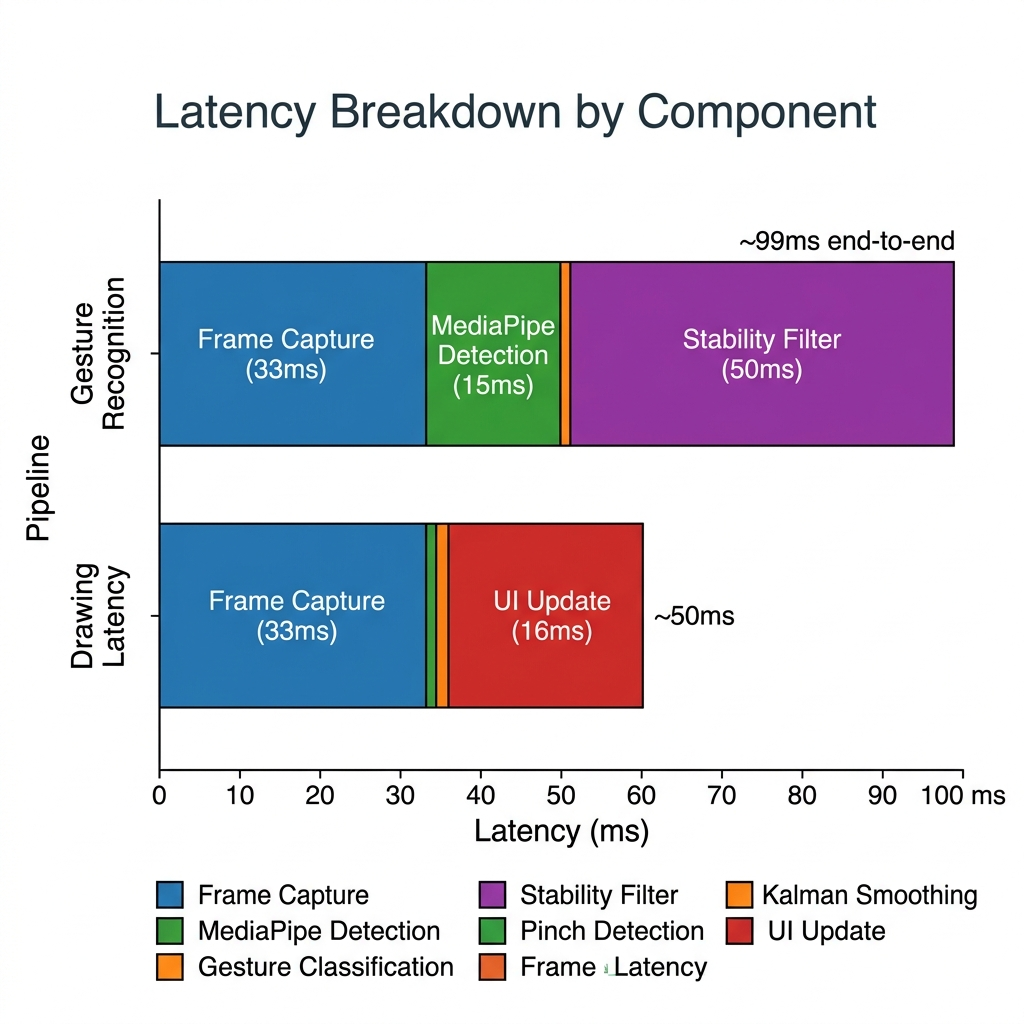
\includegraphics[width=\columnwidth]{latency_chart.png}
\caption{Latency breakdown for gesture recognition and drawing pipelines. Gesture recognition is dominated by the stability filter (by design); drawing latency is dominated by frame capture and UI updates.}
\label{fig:latency}
\end{figure}

\textbf{Gesture recognition} has an end-to-end latency of approximately 100\,ms, dominated by the intentional stability filter (5 frames $\times$ 10\,ms = 50\,ms minimum). This delay is by design---it prevents accidental triggers and makes the system feel deliberate. The actual classification takes under 1\,ms.

\textbf{Drawing latency} is approximately 50\,ms from hand movement to rendered stroke, comprising frame capture ($\sim$33\,ms at 30\,fps), pinch detection ($< 1$\,ms), Kalman smoothing ($< 0.1$\,ms), and UI update ($\sim$16\,ms at 60\,fps). Users report that drawing feels responsive and natural at this latency.

\textbf{Air writing inference} adds negligible overhead at 0.15\,ms per prediction, confirming that the ONNX Runtime deployment was the right choice over TensorFlow.

\section{Discussion}

\subsection{What Worked Well}

The modular architecture paid dividends throughout development. When we needed to switch from index-finger tracking to pinch-based tracking, only the tracker and drawing canvas modules needed changes---the gesture classifier, media engine, and UI were unaffected. Similarly, when TensorFlow proved too heavy for deployment, swapping in ONNX Runtime required changes to a single file.

The pinch gesture turned out to be a surprisingly good interaction metaphor. Users who tried the system for the first time intuitively understood ``pinch to draw, release to stop'' without any instruction. This is likely because the gesture maps to a familiar physical action (holding a pen), unlike the original index-finger pointing which has no natural ``pen up'' equivalent.

The customizable gesture mapping was initially a nice-to-have feature, but user feedback revealed it was essential. Left-handed users preferred different gesture assignments than right-handed users, and some gestures that felt natural to one person felt awkward to another. Making mappings user-configurable, rather than hardcoded, turned out to be one of the most important design decisions.

\subsection{Limitations}

We are honest about what does not work perfectly:

\begin{itemize}[leftmargin=*]
    \item \textbf{Single-hand tracking}: MediaPipe can track two hands, but we limited the system to one hand for simplicity. Two-handed gestures could enable richer interactions (e.g., pinch-to-zoom).
    \item \textbf{Lighting sensitivity}: Performance degrades in poor lighting or with strong backlighting, because MediaPipe's hand detection relies on skin color and edge features.
    \item \textbf{Air writing consistency}: Character recognition accuracy depends heavily on how consistently the user draws. Slow, deliberate strokes work well; fast, sloppy ones often confuse similar characters (e.g., ``O'' vs.\ ``0'', ``l'' vs.\ ``1'').
    \item \textbf{No word-level correction}: The system recognizes individual characters without any language model post-processing. A spell-checker or language model could dramatically improve effective accuracy.
    \item \textbf{Gesture vocabulary}: Static hand poses capture only a fraction of possible gestures. Dynamic gestures (swipe left, circular motion) could expand the vocabulary but require sequence models.
\end{itemize}

\subsection{Future Work}

Several directions could extend this work. Transformer-based sequence models~\cite{xu2023} could recognize dynamic gestures and improve air writing through attention over temporal stroke features. Multi-hand tracking would enable two-handed interaction patterns. A language model (even a simple n-gram model) for post-processing air writing output could correct common misrecognitions contextually. Finally, porting the application to mobile platforms via MediaPipe's on-device APIs could bring touchless interaction to smartphones and tablets.

\section{Conclusion}

This paper presented GestureVLC, a cross-platform touchless media player that puts three capabilities into one application: real-time gesture recognition (93.23\% accuracy, 14 classes), pinch-based air drawing with Kalman-filtered tracking, and CNN-powered character recognition with 0.15\,ms ONNX inference.

More than the numbers, we hope this work demonstrates that gesture recognition research can---and should---be packaged into applications that people actually use. The gap between a research demo and a usable tool is often not algorithmic sophistication, but engineering care: debounce logic, DLL compatibility, dark-mode styling, and the hundred small decisions that make software feel polished rather than prototype-grade.

GestureVLC is open-source and available for anyone to use, extend, or learn from. We look forward to seeing what others build on top of it.

\begin{thebibliography}{00}

\bibitem{hagrid2022} A.~Kapitanov, A.~Makhlyarchuk, and K.~Kvanchiani, ``HaGRID -- HAnd Gesture Recognition Image Dataset,'' in \textit{Proc. IEEE/CVF Winter Conf. Applications of Computer Vision (WACV)}, 2024, pp.~4460--4469.

\bibitem{mediapipe2019} F.~Zhang, V.~Bazarevsky, A.~Vakunov, A.~Tkachenka, G.~Sung, C.-L.~Chang, and M.~Grundmann, ``MediaPipe Hands: On-device Real-time Hand Tracking,'' \textit{arXiv preprint arXiv:2006.10214}, 2020.

\bibitem{breiman2001} L.~Breiman, ``Random Forests,'' \textit{Machine Learning}, vol.~45, no.~1, pp.~5--32, 2001.

\bibitem{cohen2017} G.~Cohen, S.~Afshar, J.~Tapson, and A.~van~Schaik, ``EMNIST: Extending MNIST to handwritten letters,'' in \textit{Proc. Int. Joint Conf. Neural Networks (IJCNN)}, 2017, pp.~2921--2926.

\bibitem{alam2020} M.~S.~Alam, K.~C.~Lim, and A.~Rashid, ``CNN-Based Air Writing Character Recognition System,'' \textit{IEEE Access}, vol.~8, pp.~213456--213467, 2020.

\bibitem{chen2019} X.~Chen, H.~Guo, G.~Wang, and L.~Zhang, ``Motion Feature Augmented Recurrent Neural Network for Skeleton-Based Dynamic Hand Gesture Recognition,'' in \textit{Proc. IEEE Int. Conf. Image Processing (ICIP)}, 2019, pp.~3250--3254.

\bibitem{raheja2011} J.~L.~Raheja, A.~Chaudhary, and K.~Singal, ``Tracking of Fingertips and Centres of Palm using Kinect,'' in \textit{Proc. Int. Conf. Computational Intelligence, Modelling and Simulation}, 2011, pp.~248--252.

\bibitem{mitra2007} S.~Mitra and T.~Acharya, ``Gesture Recognition: A Survey,'' \textit{IEEE Trans. Syst., Man, Cybern. C, Appl. Rev.}, vol.~37, no.~3, pp.~311--324, 2007.

\bibitem{rautaray2015} S.~S.~Rautaray and A.~Agrawal, ``Vision based hand gesture recognition for human computer interaction: A survey,'' \textit{Artif. Intell. Rev.}, vol.~43, no.~1, pp.~1--54, 2015.

\bibitem{molchanov2016} P.~Molchanov, X.~Yang, S.~Gupta, K.~Kim, S.~Tyree, and J.~Kautz, ``Online Detection and Classification of Dynamic Hand Gestures with Recurrent 3D Convolutional Neural Networks,'' in \textit{Proc. IEEE Conf. Computer Vision and Pattern Recognition (CVPR)}, 2016, pp.~4207--4215.

\bibitem{ohnbar2013} E.~Ohn-Bar and M.~M.~Trivedi, ``Hand Gesture Recognition in Real Time for Automotive Interfaces: A Multimodal Vision-Based Approach and Evaluations,'' \textit{IEEE Trans. Intell. Transp. Syst.}, vol.~15, no.~6, pp.~2368--2377, 2014.

\bibitem{pisharady2015} P.~K.~Pisharady and M.~Saerbeck, ``Recent methods and databases in vision-based hand gesture recognition: A review,'' \textit{Computer Vision and Image Understanding}, vol.~141, pp.~152--165, 2015.

\bibitem{mukherjee2019} S.~Mukherjee, S.~A.~Ahmed, D.~P.~Dogra, S.~Kar, and P.~P.~Roy, ``Fingertip Detection and Tracking for Recognition of Air-Writing in Videos,'' \textit{Expert Systems with Applications}, vol.~136, pp.~217--229, 2019.

\bibitem{xu2023} P.~Xu, X.~Zhu, and D.~A.~Clifton, ``Multimodal Learning with Transformers: A Survey,'' \textit{IEEE Trans. Pattern Anal. Mach. Intell.}, vol.~45, no.~10, pp.~12113--12132, 2023.

\bibitem{onnxruntime} ONNX Runtime Developers, ``ONNX Runtime: Cross-platform, High Performance ML Inferencing and Training Accelerator,'' 2021. [Online]. Available: https://onnxruntime.ai/

\bibitem{lecun1998} Y.~LeCun, L.~Bottou, Y.~Bengio, and P.~Haffner, ``Gradient-Based Learning Applied to Document Recognition,'' \textit{Proc. IEEE}, vol.~86, no.~11, pp.~2278--2324, 1998.

\bibitem{kalman1960} R.~E.~Kalman, ``A New Approach to Linear Filtering and Prediction Problems,'' \textit{J. Basic Eng.}, vol.~82, no.~1, pp.~35--45, 1960.

\end{thebibliography}

\end{document}
